\documentclass[12pt]{article}
\usepackage[paperwidth=8.5in,paperheight=11in,margin=1in]{geometry}
\usepackage{float}
\usepackage{lipsum}
\usepackage{parskip}
\usepackage{bbding}
\usepackage{amssymb}
\usepackage{titlesec} 
\usepackage{graphicx}
\usepackage{hyperref}
\usepackage{setspace}
\usepackage[normalem]{ulem}
\usepackage[section]{placeins}
\usepackage[toc,page]{appendix}
\newcounter{subsubsubsection}[subsubsection]
\newcommand{\tline}{\hspace{-2.3pt}$\bullet$ \hspace{5pt}}
\hypersetup{colorlinks=true, linkcolor=black, urlcolor=blue}
\setlength{\parindent}{12pt} % Indent paragraphs (automatically)

\makeatother
\makeatletter
\setlength{\@fptop}{0pt}

\begin{document}
	\begin{titlepage}
		\centering	
    
    \begin{figure}[h]
      \centering
      
\includegraphics[width=0.55\linewidth]{glassesIcon.png}
    \end{figure} 
  
  {\huge\bfseries Goofy Lights: \\ Design Specification\par}
  		\vspace{.25cm}
    
		{ \setstretch{0.2}		
      {\Large\itshape Animesh Pattanayak\\}	
      {\Large\itshape Adrian Beehner\\}
      {\Large\itshape Robert Stewert\\}	
      {\Large\itshape Joseph Leister\\}
      {\Large\itshape Andrew Butler\\}
      {\Large\itshape Megan Phelan\\}
      {\Large\itshape Seth Forrest\\}
		}		
    \vspace{.25cm}	
    
		supervised by \\
		Bruce Bolden		
    
    \vspace{.5cm} 
    
    {\scshape\Large 
      CS 383: Spring 2016 \\
      Software Engineering Semester Project
      \par}
    
    \begin{figure}[h]
      \centering
      
\includegraphics[width=0.7\linewidth]{uislogan}
    \end{figure} 
  
		\vfill		
	\end{titlepage}

	\tableofcontents
	\newpage
	
	\section{Introduction}
		\subsection{Project Summary}
  		The University of Idaho Marching Band has recently begun an experimental project to equip members of the University marching band with light-up glasses. The task described in this document is part of a semester project for the CS 383: Software Engineering class at the University of Idaho.  The project is to design and implement a graphical user interface (GUI) for the light-up glasses, known colloquially as \textit{Goofy Glasses}. 
      \\
      This GUI, written in Java, grants a user the ability to manipulate the state of each pair of glasses to create elaborate designs and patterns. This piece of software should be intuitive enough to be usable by any individual with little or no training. The program allows a user to manipulate the color and state of a single node, multiple nodes, or bulk properties of all nodes. The workspace allows the layout of more nodes than is required by the marching band, to allow for additional pairs of Goofy Glasses to be added in the future. In addition, the user is able to specify workspace dimensions up to 20 x 20, allowing for different sized shows. 
      \\
      This document lives at \url{https://github.com/GoofyGlasses-CS383-S17/Design-Specification} 
      \\
      The code for the project can be found at \url{https://github.com/GoofyGlasses-CS383-S17/GridEditor}
		
		\subsection{Document Purpose}
  		This document is a design specification for the spring 2017 CS 383: Software Engineering semester project at the University of Idaho. The purpose of this document is to outline the methodology and design of this project. It defines terms used, outlines the scope of the project, details specific design choices, and reveals changes made in the creation of the editor. 
		
		\subsection{Definition of Terms}
		\begin{itemize}
      \item \textbf{Goofy Glasses} - A pair of glasses with RGB LEDs in them and a wireless receiver. Using the grid editor, an array of glasses can light up in specific patterns.
			\item \textbf{Node} - An individual pair of Goofy Glasses, represented in the editor by a single square which can be assigned a RGB value.
			\item \textbf{IDE} - Integrated Development Environment. A tool used to write and develop a software program. The IDE chosen for this project is Eclipse.
			\item \textbf{GUI} - Pronounced "gooey", the Graphical User Interface is the front end of a program that the user interacts with.
			\item \textbf{WYSIWYG} - Pronounced "whizzy wig", this acronym stands for What You See Is What You Get. It is often associated with graphical tools that allow you to drag and drop objects in order to design a GUI, web-page, or other graphical output. 			
		\end{itemize}
		
		\subsubsection{Java JDK}
  		This program was written in Java, and required the use of the Java Development Kit (JDK). At the time of this document the current release is version 8 update 121 and can be downloaded from Oracle at \url{http://www.oracle.com/technetwork/java/javase/downloads/jdk8-downloads-2133151.html}
		
		\subsubsection{Swing}
  		Swing is a set of libraries that can be imported into Java programs in order to create a rich GUI experience without having to import all the classes and methods for the GUI individually. While there is no specific download for the Java's swing package, the following Javadoc is helpful in identifying the different classes/components that can be used. \url{https://docs.oracle.com/javase/8/docs/api/javax/swing/package-summary.html}
		
		\subsubsection{Eclipse}
  		Eclipse is a Java based IDE that allows for easy code development. It helps keeps files organized and has some built in debugging capabilities. Eclipse is used widely by the Java community and thus offers many options for third party plug-ins to assist in development. More information along with downloads of the latest version of Eclipse can be found at \url{https://eclipse.org/}
		
		\subsubsection{WindowBuilder Pro}
  		WindowBuilder Pro (\url{https://eclipse.org/windowbuilder/download.php}) is a plug-in for Eclipse that makes GUI design quicker and easier than coding from scratch. This plug-in adds a 'design' tab to Eclipse's interface that adds tools for clean WYSIWYG design. 
		
\newpage
	\section{Program Overview/Scope}
  	This software was developed with scalability in mind. The goal was to create a Framework that can be updated and scaled easily, and to some degree, efficiently. Changes throughout the development cycle required adding the basic framework(the editor itself) and various functionalities, such as different ways to interact with the editor. \\
    This program has a GUI that allows manipulation of the color and state of each node, multiple nodes simultaneously, or bulk manipulation of the entire array. Grid dimensions and number of grids are variable, yet reside at a default value unless the user specifies. \\
    It is assumed that no nodes in the grid are allowed to change places; all nodes must reside in their original location relative to other nodes. Another assumption is that the glasses themselves are already setup with a \textit{n}-node channel receiver, being able to receive and process a $3$-byte message, for RGB values.
    \\
    The program is able to run on any Operating System with Java installed, with no changes in functionality. Each OS will utilize its own specific file system properties when loading and saving configurations.
	
    \begin{figure}[ht!]
    \centering
    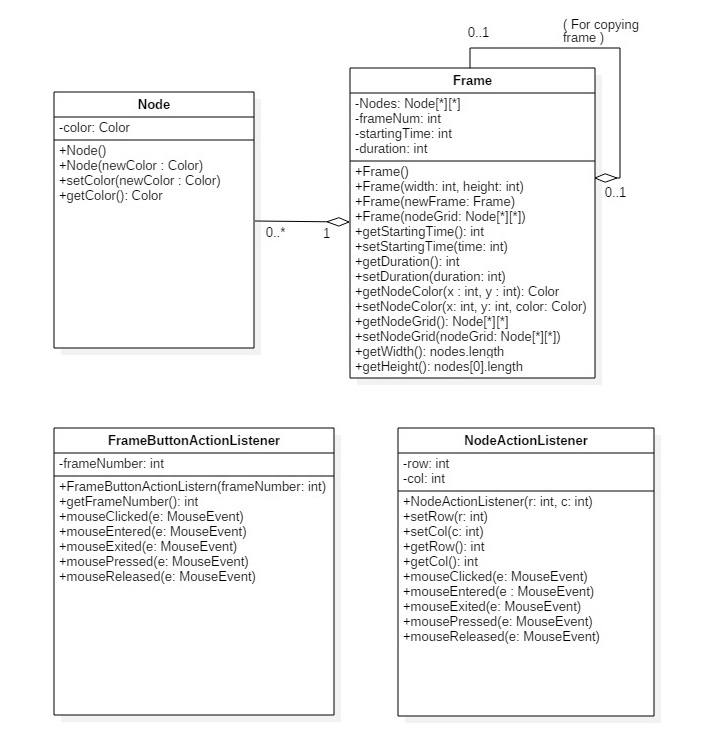
\includegraphics[width=\linewidth]{Class_Diagram_Frame_Node_and_ActionListener_Classes.JPG}
    \caption{Diagram for Frame, Node, FrameButtonActionListener, and NodeActionListener Classes}
  \end{figure}

	%----------------------------------------------------------------------------------------
	%	COMPONENT OVERVIEW
	%----------------------------------------------------------------------------------------
	\subsection {Component Overview}
    There are seven major components in the system software; Configuration Menu Bar, Grid Editor, Control Cluster, Color Picker, Presentation Timer, Frame Preview Bar, and File Generator. These components are highlighted in the figure below.
    \\
    The Configuration Menu Bar (1) provides a simple interface for setting up the size of a grid, a two-dimensional array of glasses, in addition to saving and loading a project. The Node Editor (2) provides the user with an interface to edit individual Nodes, as well as -with the use of hot keys- multiple Nodes. 
    \\
    On the top right side of the window is the Control Cluster (3). It allows the user to interact with the the nodes in various ways, described below. Beneath the control cluster is the Color Picker(4). This box contains a set of common color options, a list of recently used colors, and -by selecting the RGB tab- provides the user with the ability to generate a custom color. At the bottom of the right panel is the Presentation Timer(5). This provides the user with the ability to view and edit the frame's start time and/or duration. 
    \\
    The Frame Preview Bar(6) sits at the bottom of the interface and provides the opportunity to see a preview of the various frames in the show. The frame that is currently being edited is highlighted with a blue border, and a Right Click menu provides the user with various options. 
    \\
    The File Generator is a simple interface that allows the text representation of the animations created in the Animation Creator to be a saved to a \textit{.tan} file format. This interface lives within the File drop-down menu in the Configuration Menu Bar. 
   
  \begin{figure}[h]
    \centering
    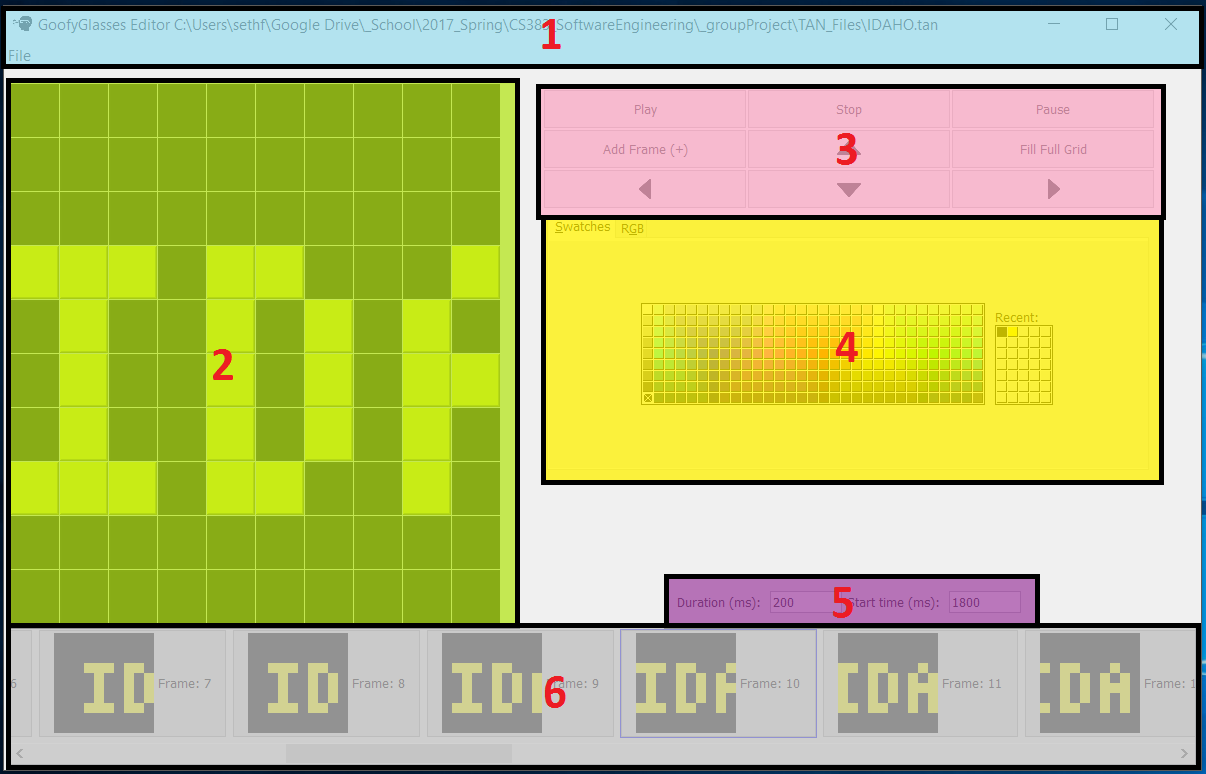
\includegraphics[width=\linewidth]{editor.png}
    \caption{
      The components of the Goofy Glasses Editor. (1) Configuration Menu Bar, (2) Grid Editor, (3) Control Cluster, (4) Color Picker, (5) Presentation Timer, and (6) Frame Preview Bar
    }
  \end{figure}

	%----------------------------------------------------------------------------------------
	%	CONFIGURATION MENU BAR
	%----------------------------------------------------------------------------------------
	\subsubsection {Configuration Menu Bar}
  	The configuration menu bar is a simple interface via a horizontal menu bar on the GUI that provides the user with various options on how they wish to manipulate the file, as well as window controls that are inherited from the OS. 
    \\
    The only input accepted is from clicking on a tab to access it's dialog boxes and displays. The topmost functions are inherited from the OS that the program is running on, and should therefore be familiar to the user. 
    \\
    A dialog box will appear when the New File option is accessed that will provide users the ability to select a dimension. Only grid dimensions will be allowed if all the $n$-nodes can fit within that space, up to and including 20x20, otherwise an error will be displayed. Also in the file option a user will be allowed to open a saved project, save the current project, or 'save as' the current project. \\
     
  	\begin{figure}[h]
  		\centering
  		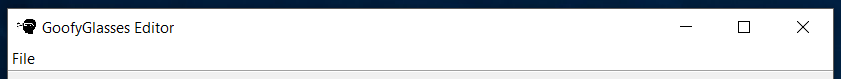
\includegraphics[width=\linewidth]{configuration_menu_bar.png}
  		\caption{The Configuration Menu Bar for the Goofy Glasses Editor.}
  	\end{figure}
	
  
   %-------------------------------------------------
  %	GRID EDITOR
  %-------------------------------------------------
  \subsubsection {Grid Editor}
    The Grid Editor component is in charge of editing all the nodes within a grid. This component handles the selection of individual or multiple nodes. The user can edit a single node by selecting a color in the Color Picker, then Left Clicking on the desired node.
    \\ 	
    The User may want to apply this color to a sub-array of nodes. For example, they may want to select a 5x5 sub-grid and change the color to green. They can accomplish this by selecting one corner of the desired sub-grid, as they would normally paint that node, then Shift+Click the diagonal corner of the sub-grid. This function is responsible for allowing the user to select up to and inclusive of the entire field. The constraint of this function is that it will only select rectangular grids.
    \\
    The final way the user may interact with the Grid Editor is to 'paint' a series of nodes. This can be accomplished by holding Ctrl down while dragging the mouse over the desired nodes. This will apply the currently selected color to any node under the mouse while Ctrl is held. 
   
  \begin{figure}[h]
    \centering
    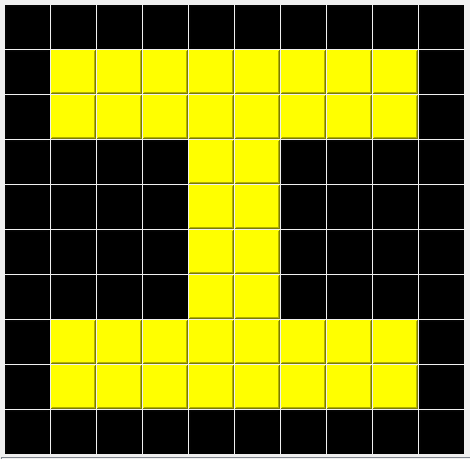
\includegraphics[width=.6\linewidth]{Grid.png}
    \caption{A 10x10 grid with the Idaho `I' painted on it. }
  \end{figure}
 

 
	%----------------------------------------------------------------------------------------
	%	CONTROL CLUSTER
	%----------------------------------------------------------------------------------------
	\subsubsection {Control Cluster}
  		The Control Cluster contains buttons that allow the user to interact with the grid and/or frames. 
      \\
      The first row of buttons allow the user to preview the show being built. ``Play" will run the show, starting at the currently selected frame, utilizing each frames time as specified in the Presentation timer. ``Stop" will stop playing the show that is currently playing and reset it to the frame that was selected when Play was pressed. ``Pause" will stop the show at the location that is being displayed when pressed. To resume the show the user must press Play again.
      \\
      The second row in the Control Cluster contains the ``Add Frame" button which will insert a blank frame after the currently selected frame. The ``Fill Full Grid" will paint all of the nodes in the currently selected frame with the currently selected color.
      \\
      The remaining four buttons in the Control Cluster are the shift buttons, identified by arrows indicating the direction in which they shift the nodes. When the user presses the ``Shift Up" button, as identified by the up arrow in the middle-most button, the entire array of nodes will shift up one cell. Any nodes that would be `pushed off' of the grid are instead wrapped around and appear on the bottom of the node editor.
      
    \begin{figure}[h]
      \centering
      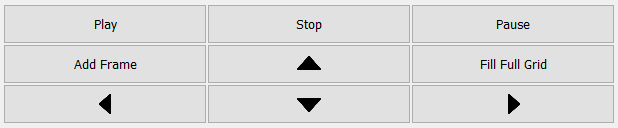
\includegraphics[width=.8\linewidth]{control_cluster.png}
      \caption{
        The Control Cluster has controls for shifting the node array in the indicated direction, as well as the ability to add a frame, color all nodes in the editor, and Play, Pause and Stop an animation 
      }
    \end{figure}
  
	%----------------------------------------------------------------------------------------
	%	COLOR PICKER
	%----------------------------------------------------------------------------------------
	\subsubsection {Color Picker}
  	The Color picker is a simplified implementation of Java's \textit{JColorChooser}. This component has two tabs; Swatches, and RGB.
    \\
    Swatches contains a wide variety of many common colors, as well as a `memory' of the most recently used colors. The user selects the color they wish to work with and the recent color pane is automatically updated.
    \\
    The RGB tab allows the user to manually specify a specific color using the Red, Green, and Blue color value boxes. Additionally the user has the option to use the sliders of graphically select a specific color.
    
  \begin{figure}[h]
    \centering
    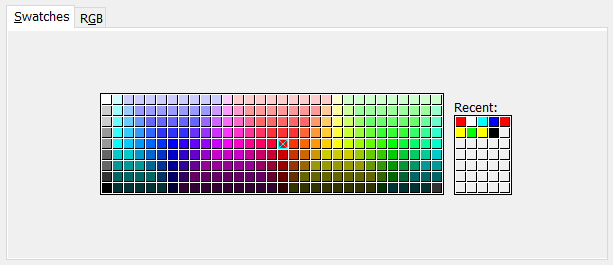
\includegraphics[width=.45\linewidth]{color_swatches.png}
    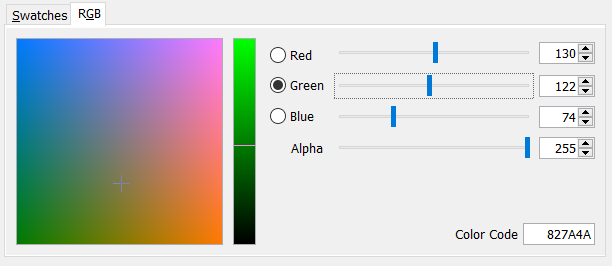
\includegraphics[width=.45\linewidth]{color_RGB.png}
    \caption{
      The Swatches picker provides many common colors. The RGB color picker allows the user to manually specify the color value.
    }
  \end{figure}
  
  
	%----------------------------------------------------------------------------------------
	%	PRESENTATION TIMER
	%----------------------------------------------------------------------------------------
	\subsubsection {Presentation Timer}
  	 The Presentation timer allows the user to create a dynamic presentation by allowing variable durations to each individual frame. The two ways to pick when a frame is activated is by specify the frame's start time, in milliseconds, or to specify the duration the frame is active. When editing either field the Goofy Lights Editor will attempt to update the time code of all following frames.
     
   \begin{figure}[h]
     \centering
     
\includegraphics[width=.6\linewidth]{presentation_timer.png}
     \caption{
       The Presentation Timer allows editing of a frame's time code.
     }
   \end{figure}
  %----------------------------------------------------------------------------------------
  %	FRAME PREVIEW BAR
  %----------------------------------------------------------------------------------------
  \subsubsection {Frame Preview Bar}
   The Frame Preview Bar is responsible for the viewing and selection of frames; saved grid formations. It provides an interface that shows the user a simple ``preview" of the current list of frames. Upon loading a \textit{.tan} file, the frame preview bar will generate a list of frames that was read in. The Frame Preview Bar also works alongside the control cluster's  ``Add Frame (+)" button, which will take the current configuration of the grid and append that frame to the current frame list. The Frame Preview Bar will then update its graphic to reflect this change.
   \\
   There are two primary inputs available. The first is to Left Click upon the frame preview for the corresponding frame, which then will have the GUI load the frame's configuration into the grid editor, the currently selected fame is highlighted with a blue border. The second is a Right Click Menu that allows the user to delete a frame, insert a frame both before an after the current frame, or duplicate the selected frame in either the next slot or at the end of the show.
   \\
   One notable secondary input is the ability to click and drag the scroll bar, provided there is more frames than can fit in the alloted space, to move through the list of frames. This preview bar has some system resource demands, as the actions described can be resource intensive, such as having the frame preview bar generate a preview for each frame. An example of the Frame Preview Bar is shown in the following diagram.
  
  \begin{figure}[ht!]
    \centering
    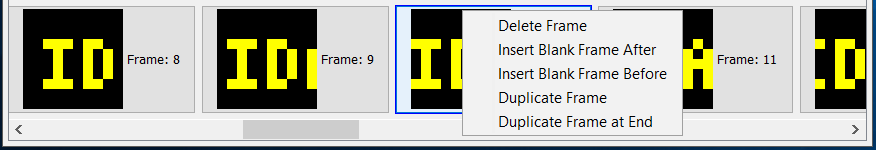
\includegraphics[width=\linewidth]{frame_preview.png}
    \caption{The frame preview bar with frame 10 selected, displaying the Right Click menu.}
  \end{figure}



  %----------------------------------------------------------------------------------------
  %	FILE GENERATOR
  %----------------------------------------------------------------------------------------
  \subsubsection {File Generator}
    This component is responsible for outputting a text representation of the animations created in the program. The file must be in the \textit{.tan} format for use by the glasses and for future editing via this program.
    \\
    Each node in the grid editor is represented by a set of three 8-bit numbers that correspond to RGB values. 
  
  
  	\begin{figure}[ht!]
  		\centering
  		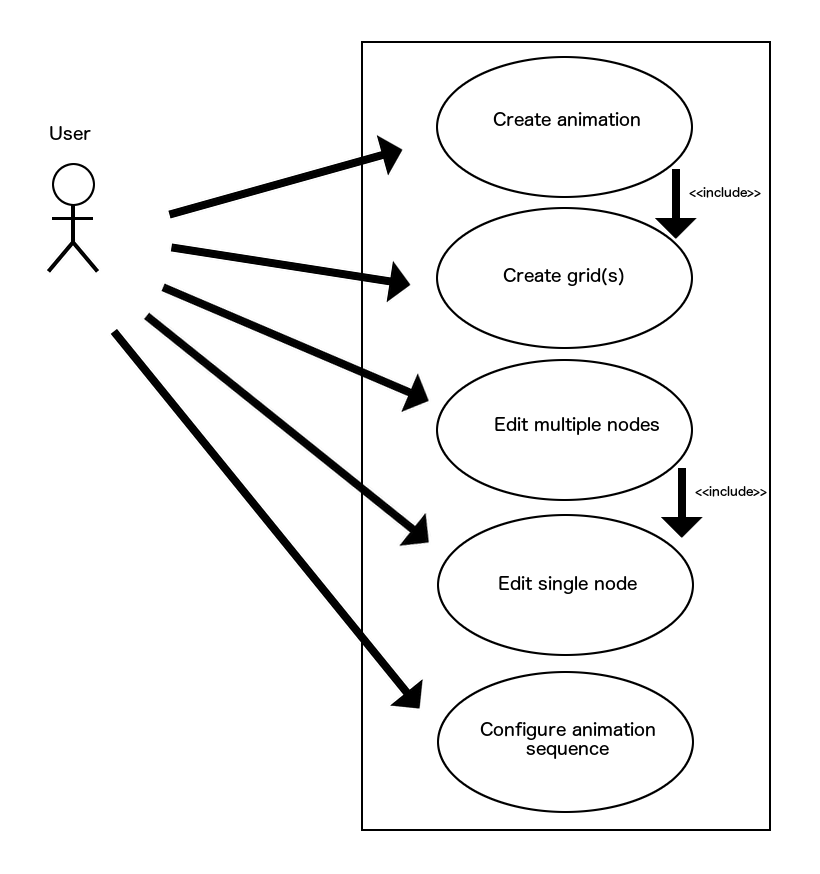
\includegraphics[width=0.8\linewidth]{Relationship_Use.png}
  		\caption{Use Case for interacting with the editor.}
  	\end{figure}
	\clearpage	
\newpage

	\section{Design Decisions}
    When planning this project, several decisions were made to limit the scope and complexity of the final product. These decisions are detailed below. 
    
  	\subsection{\textit{.tan} File}
	  	The user is able to save and load \textit{.tan} files via the GUI interface. A \textit{.tan} file is a text file with the following format.
      \\
      The first line indicates the program version number. The next line specifies the name of an audio file(or states noAudioFile) which is to be loaded by the \textit{.tan} player. The third and fourth line are currently unused. These lines remain to maintan backwards compatability with legacy editors, players, and shows. The fifth line uses three integers to specify the number of frames contained in the show and the dimensions of the grid. 
      \\
      Then starting with the sixth line, the \textit{.tan} file stores the individual frames, with the first line of the "frame" stating the frame's time code in milliseconds. Then all the remaining lines represent each row, thus if the grid size was $10 \times 10$, there would ten additional lines. Each line then has $3 \times number\_of\_columns$ values allowing for RGB values to be stored for each node.
      \\
      This will generate $10_{columns} \times 3_{color\_values}=30$ integers for each line, where 3 of those values are the RGB for one cell/node. Saving the current frame configuration in the GUI will convert the information into a \textit{.tan} file. This allows the user to save and load files as needed. From the GUI these \textit{.tan} files can be loaded to display the state of the saved grid, updating grid dimensions as specified by the file, and displaying the first frame.
  	
  	\subsection{Language Decisions}
    	Java is the primary tool used in this project. It is convenient as it works easily across multiple platforms, is very readable, and provides its own graphics package. 
      \\
      Swing is a Java graphics package designed to make APIs that work and look the same across all Java platforms. It is built into the language so no external libraries are needed. The use of Qt integration for Java, Qt Jambi, was considered but ultimately dismissed as that this would add complexity without providing functionality. 
      
  	\subsection{Constant Positions}
    	Each node must maintain a constant position relative to one-another. If the nodes are free to move around during a performance, and the software needed to support such moving, the complexity would increase drastically. Only by limiting the editor to a static configuration of nodes does this project become reasonable. 
      
  	\subsection{Grid Scalability}
    	The user is able to set the grid dimensions to be used for the performance they are creating. A solid rectangular grid will be the only supported configuration. The user will account for any unused nodes in the rectangle when designing characters or animations. 
      \\
      Limiting the grid to a rectangle dramatically reduces the amount of options the editor needs to support, and there are few cases in which a non-rectangular array is desirable.  	
      
\newpage

\begin{appendices}
	\section{Timeline}
  This was the timeline for UIdaho's Spring 2017 CS 383: Software Engineering class.\\
	{ \setstretch{2.0}		
  	\scalebox{1}{  		
  		\begin{tabular}{r |@{\tline} l}  			
  			March 6  & Design Specifications Version 1          \\			
  			March 21 & Begin Sprint 1 of GoofyLights            \\			
        March 23 & Develop GUI for Single Node Editor       \\			
        March 25 & File I/O for Single Node                 \\			
  			March 27 & Unit Testing for Sprint 1                \\			
        March 30 & End Sprint 1 and Begin Sprint 2          \\			
  			April 4  & File I/0 for GUI                         \\			
  			April 6  & Begin Development of Frame Editor        \\			
  			April 11 & End Sprint 2 and begin Sprint 3          \\			
  			April 13 & Refine Frame Editor                      \\
  			April 16 & End Sprint 3 and begin Final Sprint      \\
        April 18 & Right-Click Menu in Scrub Bar            \\				
  			April 20 & Refine Color Palate                      \\			
  			April 25 & System Testing                           \\			
        April 27 & Progress Report Presentation             \\			
  			April 31 & Preparation for Final Presentation       \\			
  			May 2    & GoofyLights Final Presentation           \\					
        May 5    & GoofyLights Documentation Preperation    \\				
        May 9    & Submit Final Revision and Documnetation  \\
  		\end{tabular}  		
  		}  	
	}
  
  \section{Sprint 1}
    In the initial development sprint the team created the original version of this document and laid the groundwork for the Editor. Much of the work put into this sprint was dedicated to design decisions and familiarization with Java and it's associated tools.
    
  \section{Sprint 2}
    %----------------------------------------------------------------------------------------
    %	APPENDIX A Content - Sample Code/Work Done
    %----------------------------------------------------------------------------------------
    \subsection{Changes/Updates}
    The changes made to the Design Specification was relatively small. Most of the work done is Sprint 2 went into the product itself. These changes are listed below.
    
    %----------------------------------------------------------------------------------------
    %	Frame Preview Bar
    %----------------------------------------------------------------------------------------
      \subsubsection{Updating the Diagram for Grid Editor}
        The change made to the diagram for the Grid Editor was to reconfigure the diagrams to accurately represent the current build of the system for the second sprint. The Color Class was removed from the diagram as the team opted to utilize Java's own built in Color Class. Two new classes were added in the diagram, a FrameButtonActionListener class, which does as it is named, and utilized to handle actions made to the "Frame Button" in the GUI. The other class was the NodeActionListner, which also performs as it is described, handling the button press of a node in the GUI. These diagrams thus were updated and reflected in the updated Design Specification for Sprint 2.
    
    %----------------------------------------------------------------------------------------
    %	Frame Preview Bar
    %----------------------------------------------------------------------------------------
      \subsubsection {Updating the Timeline}
        The timeline was edited to reflect the progress the team has currently made since Sprint 2 and also display the goals the team hopes to accomplish in the following sprints. Originally, we had not exactly planned for a frame editor (which include the frame preview bar), but that is now reflected in the timeline, but since it is not done, it was moved to be completed at a later sprint. The Mulit Node Editor is the next goal as well, since the Single Node Editor is fully functioning now, as well as most  of the GUI elements. The timeline reflects the idea that due to the success of the team's progress, there will be additional time to add or edit features, however this is not set in stone as difficulties in the future may arise.

    
    %----------------------------------------------------------------------------------------
    %	APPENDIX B Content - Sample Code/Work Done
    %----------------------------------------------------------------------------------------
    \subsection{Added Sections}
      Only one section was required to be added to Sprint 2, which was the TAN file section. These section(s) are further discussed below.
    
    %----------------------------------------------------------------------------------------
    %	Frame Preview Bar
    %----------------------------------------------------------------------------------------
      \subsubsection{TAN File Section}
        The TAN file section was only just implemented into the Design Specification under Design Decisions due to the team not having the full picture of the requirements of the TAN file until the end of the last sprint. The TAN file section briefly explains the purpose of the TAN file, as well as providing a brief description of the components that make up the the TAN file. These components are then explained to be utilized so that the editor can read in files, and correctly output them to the GUI, as well as having the editor write out to files, allowing users to save these TAN files. The section was fairly extensive at explaining the properties of the TAN file and its functionality within the scope of the project.
    

    
    %----------------------------------------------------------------------------------------
    %	APPENDIX C Content - Diagrams for First Development Sprint
    %----------------------------------------------------------------------------------------
    \subsection{New/Changed Diagrams for Update}
      The Following are diagrams were created/updated for relevancy in the updating the Design Specification for the second sprint, these diagrams are presented in the following sections below.
    
    %----------------------------------------------------------------------------------------
    %	CLASS DIAGRAM FOR COLOR, NODE, AND FRAME CLASS
    %----------------------------------------------------------------------------------------
      \subsubsection {Class Diagram for Grid Editor}
        The Class Diagram below in Figure displays the structure of the Grid Editor (so far), in which the Color, Node, and ActionListener classes holds the main mechanism of the Gird Editor, also showing the relationships between these classes. This has been updated from the previous sprint, by removing the Color class (utilizing Java's default Color class) and adding the NodeActionListener class and FrameButtonActionListener class. The diagram is shown in the figure below.
      
      \begin{figure}[h]
        \centering
        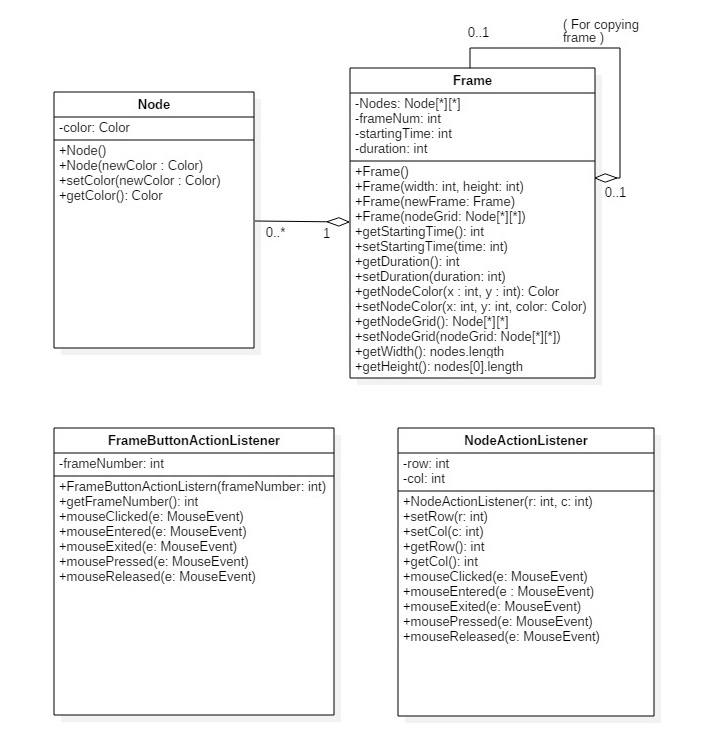
\includegraphics[width=.4\linewidth]{Class_Diagram_Frame_Node_and_ActionListener_Classes.JPG}
        \caption{Class Diagram of Grid Editor \label{overflow}}
      \end{figure}
    
    %----------------------------------------------------------------------------------------
    %	CLASS DIAGRAM FOR COLOR, NODE, AND FRAME CLASS
    %----------------------------------------------------------------------------------------
      \subsubsection {Frame Preview Bar Diagram}
        The diagram in the figure below displays the structure of the Frame Preview Bar, which contains a list of frames, which have images to show the frame's configuration. There also exists a scroll bar as shown, which allows the user to scroll to show other frames. This diagram was mainly added to present the user with a visual cue to how the Frame Preview Bar should function. The diagram is shown in Figure 2 below.
      
      \begin{figure}[ht!]
        \centering
        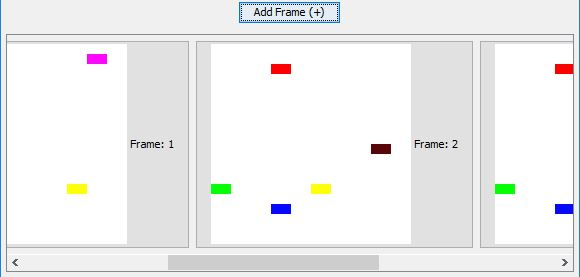
\includegraphics[width=.6\linewidth]{potoFramePre.JPG}
        \caption{Diagram of Frame Preview Bar \label{overflow}}
      \end{figure}
    
    %----------------------------------------------------------------------------------------
    %	CLASS DIAGRAM FOR COLOR, NODE, AND FRAME CLASS
    %----------------------------------------------------------------------------------------
      \subsubsection {Grid Editor Diagram}
        The diagram in the figure below displays the structure of the Grid Editor in regards to the second sprint. This was shown to display the progress made on the Grid Editor GUI since the first sprint. The Grid Editor now displays a color when the user enter the RGB values of that color in the node dialog box. This effect was supposed to be focal point of the diagram. The diagram in shown in Figure 3 below.
      
      \begin{figure}[ht!]
        \centering
        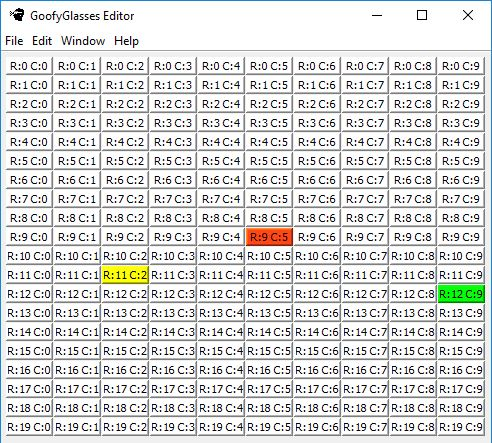
\includegraphics[width=.4\linewidth]{protoGrid.JPG}
        \caption{Diagram of Grid Editor \label{overflow}}
      \end{figure}
    
  
    
   \section{Sprint 3} 
      %----------------------------------------------------------------------------------------
      %	APPENDIX A Content - Sample Code/Work Done
      %----------------------------------------------------------------------------------------
      \subsection{Changes/Updates}
        The changes made to the Design Specification was relatively small. These changes are listed below.
      
      %----------------------------------------------------------------------------------------
      %	Frame Preview Bar
      %----------------------------------------------------------------------------------------
        \subsubsection {Updating the Diagram for Grid Editor}
          The grid editor diagram was updated to reflect the changes made to it, namely a color picker was added to the right side of the Grid Editor, the text was removed from the buttons, and a set of translation buttons was added to shift patterns around on the frame. See figure 1 below.
        
        \begin{figure}[ht!]
          \centering
          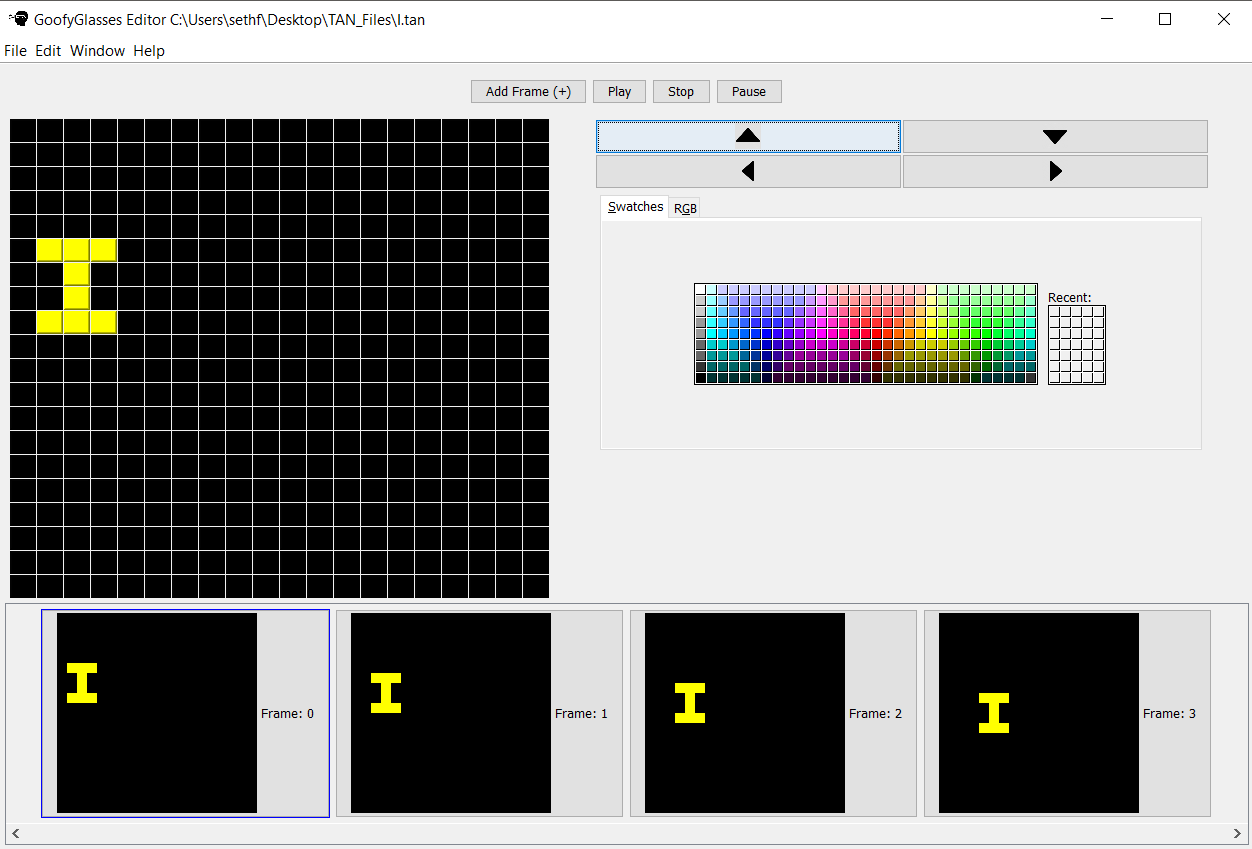
\includegraphics[width=.7\linewidth]{gridEditor_ColorPicker.PNG}
          \caption{Diagram of Grid Editor}
        \end{figure}
      
      %----------------------------------------------------------------------------------------
      %	Frame Preview Bar
      %----------------------------------------------------------------------------------------
        \subsubsection {Updating the Time-line}
          The time-line was edited to reflect the progress made since Sprint 2 and also display goals for the following sprint. The time-line now properly indicates the completion and removal of several objectives. It accurately shows that refinements were made to the Grid Editor and the scrub bar, as well as an indication that there will no longer be a multi-node editor. The time-line now also lists the addition of a progress report presentation.
      
      
      %----------------------------------------------------------------------------------------
      %	APPENDIX B Content - Sample Code/Work Done
      %----------------------------------------------------------------------------------------
      \subsection{Updated Sections}
        The Single and Multi-Node grid editor sections were removed to reflect the change to using a single Grid Editor. These section(s) are further discussed below.
      
      %----------------------------------------------------------------------------------------
      %	Frame Preview Bar
      %----------------------------------------------------------------------------------------
        \subsubsection {Grid Editor}
          The Single and Multi-Node Editor sections were removed to indicate the change in functionality of the design. This new design is a single Grid Editor with a color picker on the side, where there will eventually be the ability to Shift-Click a second node and a section of nodes will be selected to change the color.
      
        \begin{figure}[ht!]
          \centering
          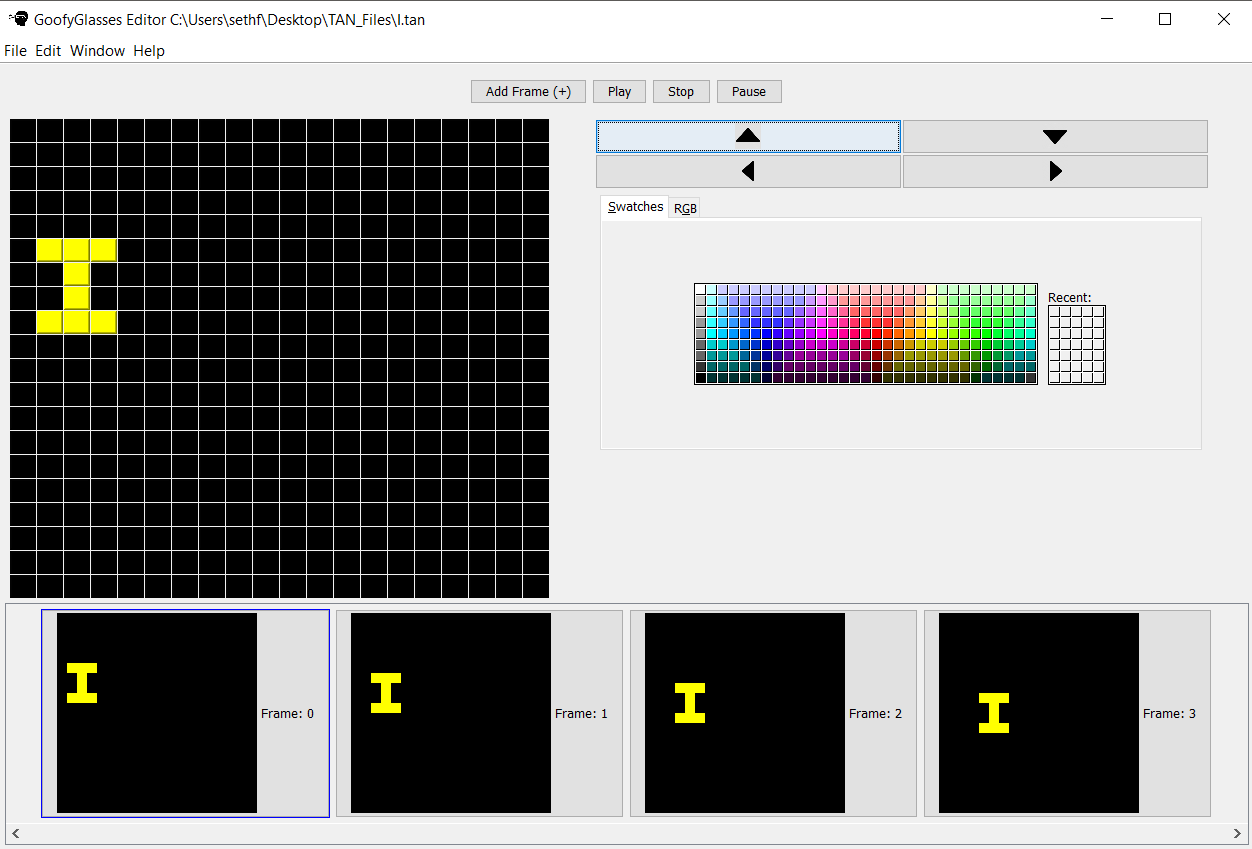
\includegraphics[width=.6\linewidth]{gridEditor.PNG}
          \caption{Diagram of Grid Editor}
        \end{figure}
      
      
      %----------------------------------------------------------------------------------------
        \subsubsection {Frame Preview Bar}
          The image below shows the right-click menu on the scrub bar. Most of the functionality is implemented in this menu and it adds a great deal of user-friendlyness to the interface.
        
        \begin{figure}[ht!]
          \centering
          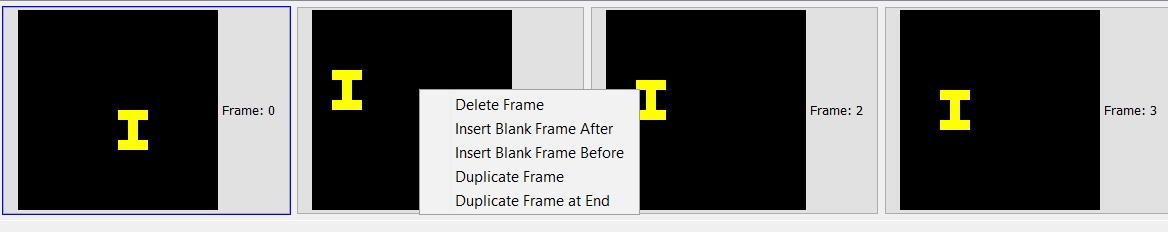
\includegraphics[width=.8\linewidth]{rtClick.PNG}
          \caption{Image of the Frame Preview Bar's Right-Click Menu}
        \end{figure}
      
      % Create new Page (NEED TO USE clearpage because we have pictures that will affect it!)
      \clearpage
      
      
      
      \section{Final Sprint} 
      %----------------------------------------------------------------------------------------
      %	APPENDIX A Content - Sample Code/Work Done
      %----------------------------------------------------------------------------------------
        \subsection{Changes/Updates}
          The final sprint focused first on getting the Editor presentation worthy, then polishing the editor and the documentation for submission. Much of the final documentation was re-written in order to accurately reflect the actual implementation of the ideas in the editor.
        
        %----------------------------------------------------------------------------------------
        %	Frame Preview Bar
        %----------------------------------------------------------------------------------------
          \subsubsection {Grid Editor Diagram and Documentation}
            The grid editor went through drastic changes throughout the course of this project, both philosophical and physical. The documentation was updated to accurately reflect the actual implementation.
          
        
        %----------------------------------------------------------------------------------------
        %	APPENDIX B Content - Sample Code/Work Done
        %----------------------------------------------------------------------------------------
        \subsection{Updated Sections}
          A Large portion of this document was updated or rewritten in alignment with what is actually implemented in the Editor.
          
          %----------------------------------------------------------------------------------------
          %	Frame Preview Bar
          %----------------------------------------------------------------------------------------
          \subsubsection {Grid Editor}
            Most of section 2 - Program Overview/Scope was either highly edited or entirely rewritten.  This includes adding many new graphics that accurately represent the current implementation of the Editor.
            \\
            Of the seven components in section 2, the Control Cluster, Color Picker, and Presentation Timer sections did not exist in previous versions of this document. Much of the other four sections required rewrites as well.
        
        
        %----------------------------------------------------------------------------------------
        \subsubsection {Appendicies}
          With the exception of appendix A, the timeline, the appendices were not previously part of this document and instead existed as separate documents. 
          \\
          Appendix A was moved from the parent document into an appendix to reflect its status as legacy information.
          \\
          Appendix B did not previously exist, and is merely a statement that the first spring involved the initial creation of the document.
          \\
          Appendix C and D was the import and formatting of previously stand-alone documents. Little work was done on these documents other than formatting so as to preserve the historical accuracy of those documents.
          \\
          For Appendix E this summary was created to reflect the changes in the documentation.
      
      % Create new Page (NEED TO USE clearpage because we have pictures that will affect it!)
      \clearpage

    
  \end{appendices}

\end{document}
